\documentclass[14pt]{beamer}
\usepackage{lmodern}
\usepackage[brazil]{babel}
\usepackage{cmap}           
\usepackage[utf8]{inputenc} % Determina a codificacao utiizada

\title{\emph{Streaming algorithms}}
\author{Juan Lopes}
\date{\today}

\usefonttheme{serif}
\DeclareMathSizes{20}{20.5}{10}{10}
\makeatletter

\setbeamercolor{normal text}{fg=white,bg=black}
\setbeamercolor{alerted text}{fg=white}
\setbeamercolor{example text}{fg=white}

\setbeamercolor{structure}{fg=white}
\setbeamercolor{background canvas}{parent=normal text}
\setbeamercolor{background}{parent=background canvas}
\makeatother

\centering

\begin{document}
\begin{frame}
    \maketitle
\end{frame}

\begin{frame}
    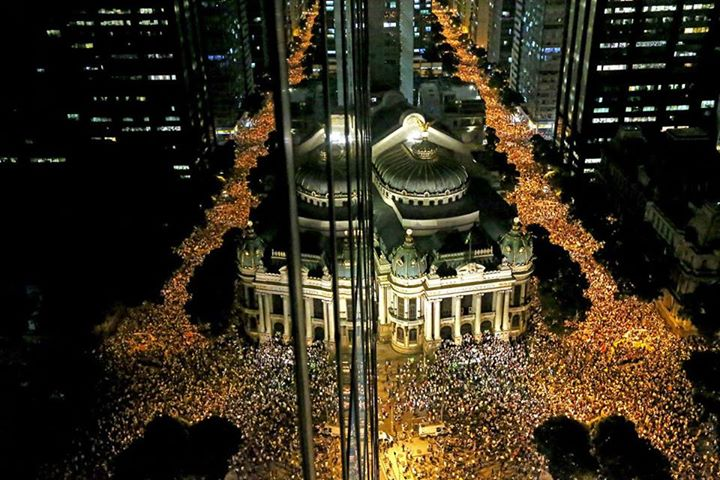
\includegraphics[scale=0.4]{figures/riobranco.jpg}

    \smallskip
    
     300 mil?
\end{frame}

\begin{frame}
    Bloom Filters \\ {\tiny\cite{bloom1970space}}

    \bigskip

    Count-Min Sketch \\ {\tiny\cite{cormode2004improved}}
    
    \bigskip
    
    HyperLogLog Sketch \\ {\tiny\cite{flajolet2008hyperloglog}}
\end{frame}

\begin{frame}
I had a big data problem, then I thought: ``I know, I'll use a {\bf bloom filter}''. 

\bigskip

Now I'm not sure how many problems I have, but {\bf I know which ones I don't.}
\end{frame}




\begin{frame}{Referências}
\fontsize{8}{2}
\bibliographystyle{apalike}
\bibliography{bibliography}
\end{frame}

\end{document}